\chapter{Реализация и тестирование}
\noindent\indent В ходе разработки написано 7000 строки кода на языке C++,
98 строк кода на шейдерном языке GLSL. Проведены численные эксперименты.
\section{Тестирование методов оптимизации}
\noindent Для проверки правильности реализации методов, они были протестированы на
нескольких известных функциях: линейной, сферической и функции Розенброка.\par
\noindentКоличество аргументов: 5.\par
\noindentКоличество экспериментов: 500.\par
\begin{table}[ht]
\centering
\resizebox{\textwidth}{!}{\begin{tabular}{|l|c|c|c|}
    \hline
    Целевая функция-Алгоритм & Градиентный метод   & Генетический алгоритм & Алгоритм Нелдера-Мида \\ \hline
    Линейная функция         & 0                   & 0                     & 0                     \\ \hline
    Сферическая функция      & 0                   & 0                     & 0                     \\ \hline
    Функция Розенброка       & 1                   & 0.2                   & 0.3                   \\ \hline
\end{tabular}}
\caption{Результаты тестирования алгоритмов оптимизации}
\end{table}\par
\chapter{Вычислительный эксперимент}
\section{Описание эксперимента}
\noindent\indent В рамках вычислительного эксперимента было решено протестировать
систему на модели движения КА при данных начальных условиях:\par
\noindent Кеплеровы элементы орбиты:
\begin{itemize}
    \item $p = 7091000$ $(\text{м})$,
    \item $e = 0.01$,
    \item $\omega = 40^\circ$,
    \item $i = 65^\circ$,
    \item $\Omega = 45^\circ$,
    \item $\tau^* = 0$.
\end{itemize}
    Параметры солнечного паруса:
\begin{itemize}
    \item $\rho = 0.9$,
    \item $B_f = B_b = 2/3$,
    \item $s = 0.9$,
    \item $e_f = 2$,
    \item $e_b = 0.1$,
    \item Площадь паруса: 40 ($\text{м}^2$),
    \item $\vec{n} = (0, 0, 1)^T$.
\end{itemize}
Параметры генетического алгоритма:
\begin{itemize}
    \item Количество поколений: 50,
    \item Размер популяции: 50,
    \item Количество скрещиваний в поколении: 30,
    \item Количество мутаций в поколении: 5.
\end{itemize}
Параметры алгоритма Нелдера-Мида:
\begin{itemize}
    \item Количество итераций: $300$.
\end{itemize}\par
\noindent Метод интегрирования: метод Рунге-Кутты четвертого порядка.\par
\noindent Максимальное изменение углов ориентации КА относительно СКО: $1^\circ$.\par
\noindent Шаг интегрирования: 1 сек.\par
\noindent Шаг оптимизации: 10 сек.\par
\noindent Интервал времени: 8600 сек.\par
\noindent Сравнительный анализ делается на основе значения высоты орбиты при
стабилизированной системе координат спутника (ССК совпадает с ОСК).
\section{Результаты}
\noindent\indent По результатам эксперимента, выявлено, что наилучший результат
показывает алгоритм Нелдера-Мида со средним приростом в высоте 2460.7764 (м). Менее
результативным оказался генетический алгоритм со средним приростом в 945.2875 (м).
\begin{figure}[h]
  \centering
  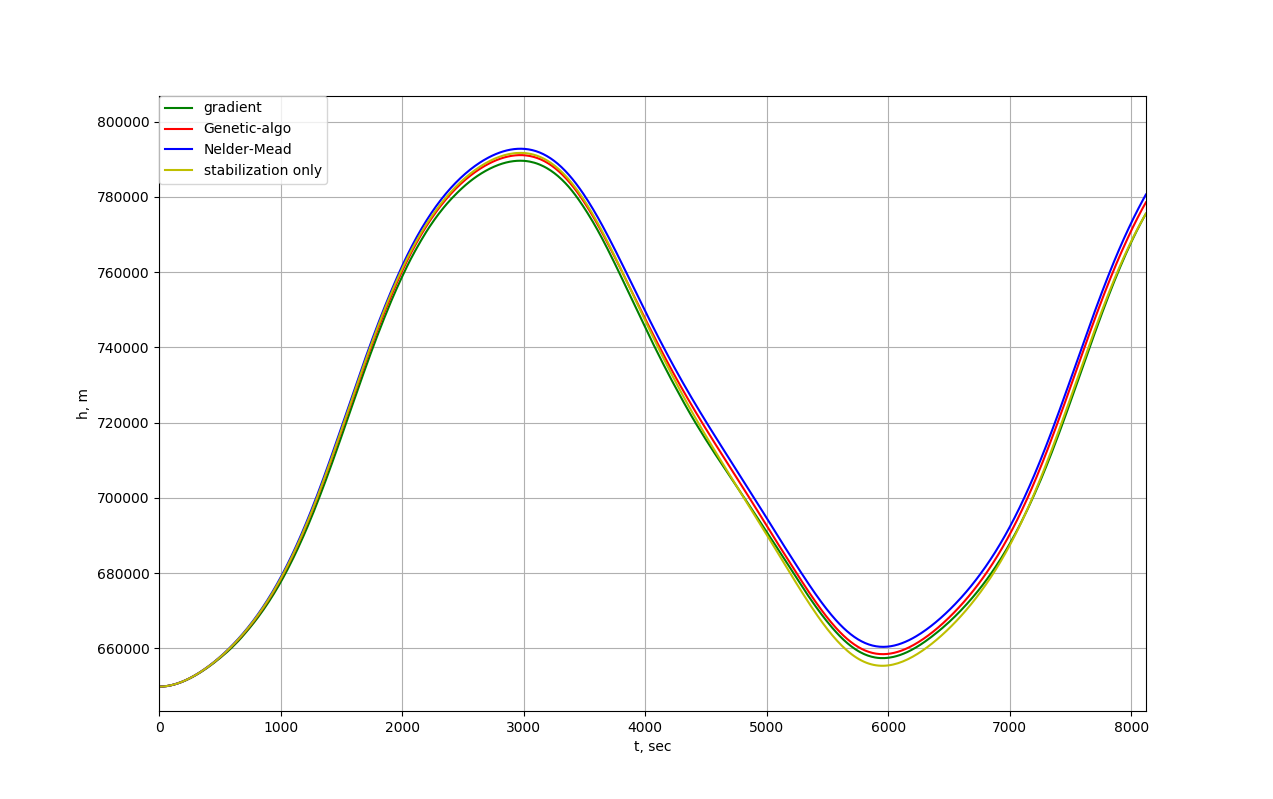
\includegraphics[width=0.8\textwidth]{FullModelFigureRadius}
  \caption{Зависимость изменения высоты орбиты от ориентации спутника}
  \label{fig:KeplerParams2Angles}
\end{figure}\par
\begin{figure}[h]
  \centering
  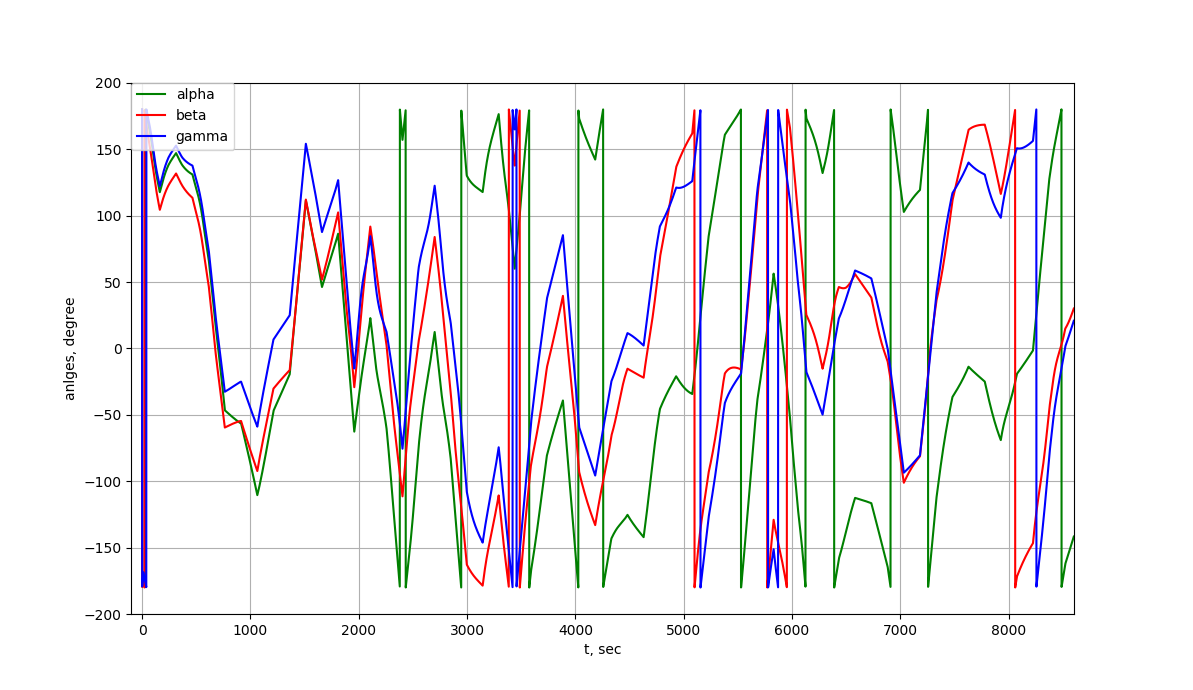
\includegraphics[width=0.8\textwidth]{FullModelFigureAnglesGradient}
  \caption{Зависимость углов ориентации спутника от высоты орбиты при использовании
  градиентного метода}
  \label{fig:KeplerParams2Angles}
\end{figure}\par
\begin{figure}[h]
  \centering
  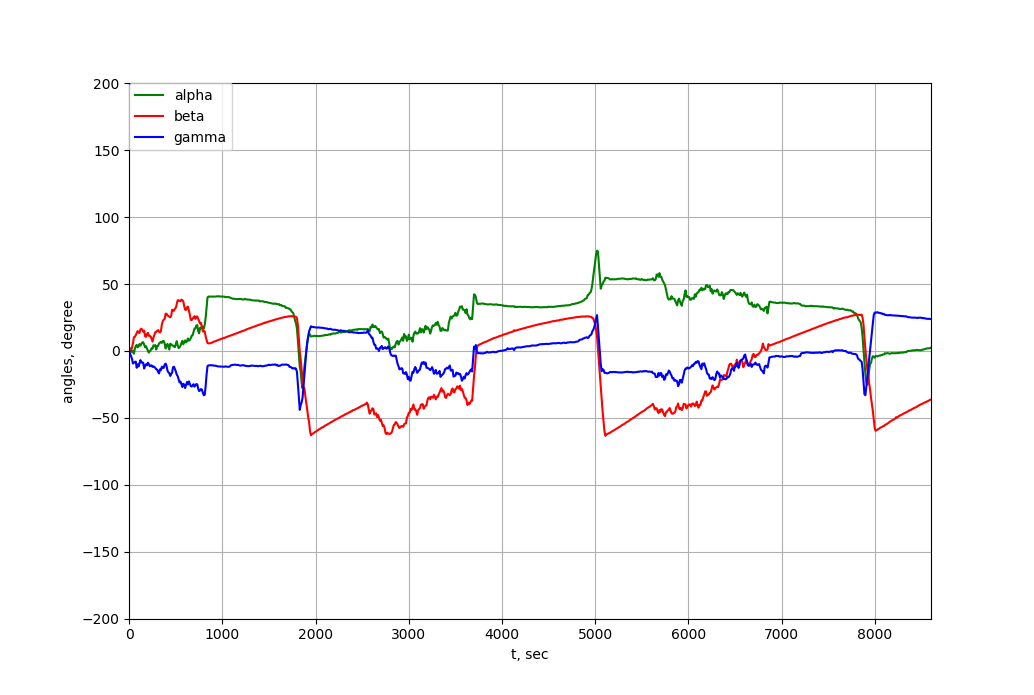
\includegraphics[width=0.8\textwidth]{FullModelFigureAnglesGA}
  \caption{Зависимость углов ориентации спутника от высоты орбиты при использовании
  генетического алгоритма}
  \label{fig:KeplerParams2Angles}
\end{figure}\par
\begin{figure}[!h]
  \centering
  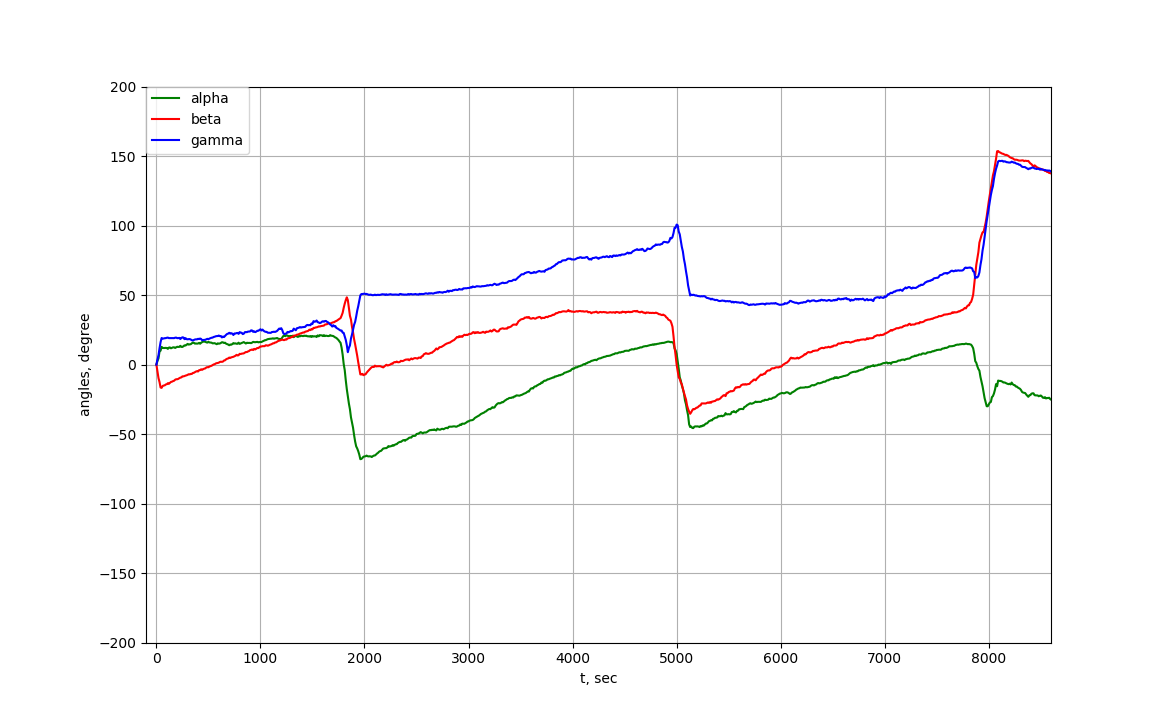
\includegraphics[width=0.8\textwidth]{FullModelFigureAnglesNM}
  \caption{Зависимость углов ориентации спутника от высоты орбиты при использовании
  алгоритма Нелдера-Мида}
  \label{fig:KeplerParams2Angles}
\end{figure}
\clearpage
